\begingroup
	\pgfdeclarelayer{background layer}
	\pgfdeclarelayer{lineas}
	\pgfsetlayers{background layer,lineas,main}
	\tikzstyle{zero}=[circle,draw=black,fill=white,inner sep=0pt,minimum size=3.5mm]
	\tikzstyle{one}=[circle,draw=black,fill=black,inner sep=0pt,minimum size=2.5mm]
	\tikzstyle{two}=[circle,draw=black,fill=gray,inner sep=0pt,minimum size=2.5mm]
	\newcounter{antip}
	\newcounter{bro}
	\newcounter{vert}
		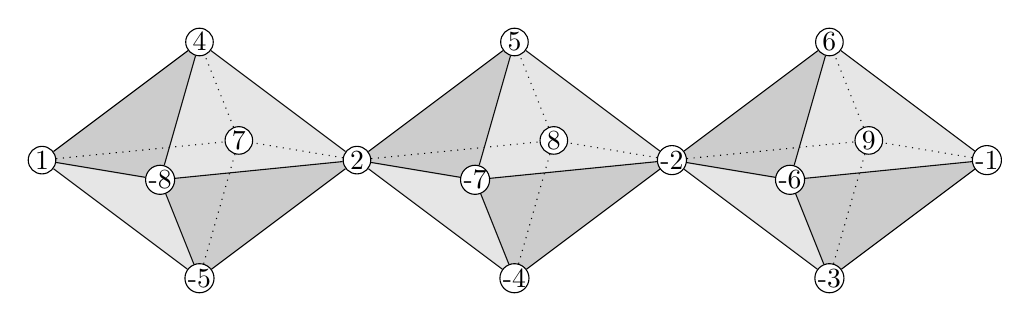
\begin{tikzpicture}
			\foreach \a/\c/\e/\d in {0/0/0/0,1.5/2/200/0,.25/2.5/250/0,-.25/1.5/150/0,-1.5/2/200/1}
			{
				\foreach \b in {0,4,8}
				{
					\stepcounter{vert}
					\stepcounter{antip}
					\ifnum \value{vert}<3
					\stepcounter{bro}				
					\node  (\b_\e_\d) at (\b+\c,\a) [zero] {$\theantip$};
					\else
					\ifnum \value{vert}<10
					\stepcounter{bro}
					\ifnum \value{vert}=3
					\node  (\b_\e_\d) at (\b+\c,\a) [zero] {-$2$};
					\else
					\setcounter{antip}{\value{vert}-1}
					\node  (\b_\e_\d) at (\b+\c,\a) [zero] {$\theantip$};
					\fi
					\else
					\addtocounter{bro}{-1}
					\node  (\b_\e_\d) at (\b+\c,\a) [zero] {-$\thebro$};
					\fi
					\fi
				}
				
			}
			\addtocounter{antip}{1}
			\node (12_0_0) at (12,0) [zero] {-$1$};
			
			\begin{pgfonlayer}{lineas}
				\foreach \b in {0,4,8}
				{
					\foreach \e/\d in {200/0,150/0,200/1}
					{
						\draw (\b_0_0) -- (\b_\e_\d);
					}
					\draw [dotted] (\b_0_0) -- (\b_250_0);
				}
				\foreach \b/\a in {4/0,8/4,12/8}
				{
					\foreach \e/\d in {200/0,150/0,200/1}
					{
						\draw (\b_0_0) -- (\a_\e_\d);
					}
					\draw [dotted] (\b_0_0) -- (\a_250_0);
				}
				\foreach \b in {0,4,8}
				{
					\draw (\b_200_0)--(\b_150_0);
					\draw (\b_150_0)--(\b_200_1);
					\draw [dotted] (\b_200_1)--(\b_250_0);
					\draw [dotted] (\b_250_0)--(\b_200_0);
				}
				\foreach \b in {0,4,8}
				{
					\fill[black,opacity=0.2] (\b+0,0)--(\b+2,1.5)--(\b+1.5,-.25);
					\fill[black,opacity=0.2] (\b+4,0)--(\b+2,-1.5)--(\b+1.5,-.25);
				}
				\foreach \b in {0,4,8}
				{
					\fill[gray,opacity=0.2] (\b+0,0)--(\b+2,-1.5)--(\b+1.5,-.25);
					\fill[gray,opacity=0.2] (\b+4,0)--(\b+2,1.5)--(\b+1.5,-.25);
				}
			\end{pgfonlayer}	
		\end{tikzpicture}
	%\label{fig:eg_torus}	
\endgroup